\begin{apendicesenv}


\chapter{Relatório KanbanFlow}
\label{sec:kanban}

\begin{figure}[h!]
\centering
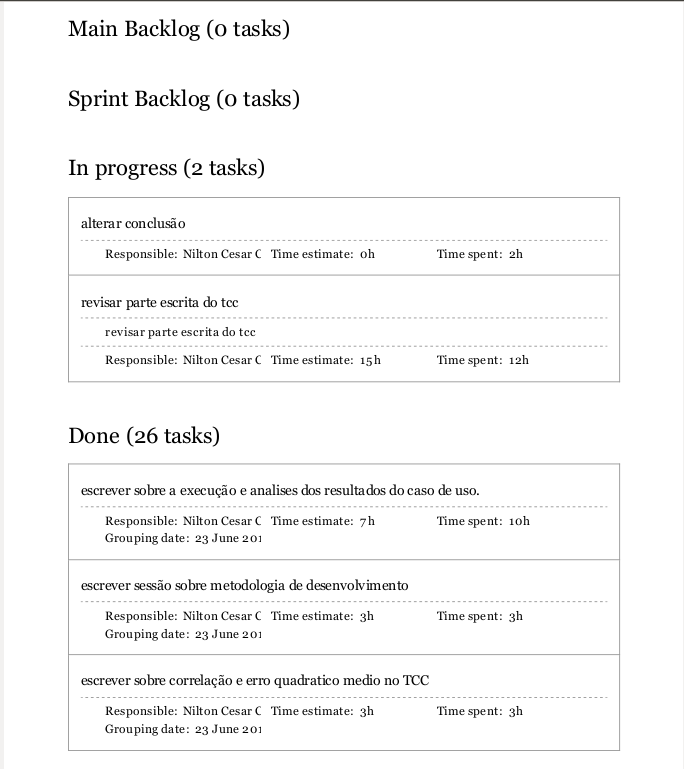
\includegraphics[keepaspectratio=false,scale=0.70]{figuras/figuras_nilton/kanban1.png}
\end{figure}

\begin{figure}[h!]
\centering
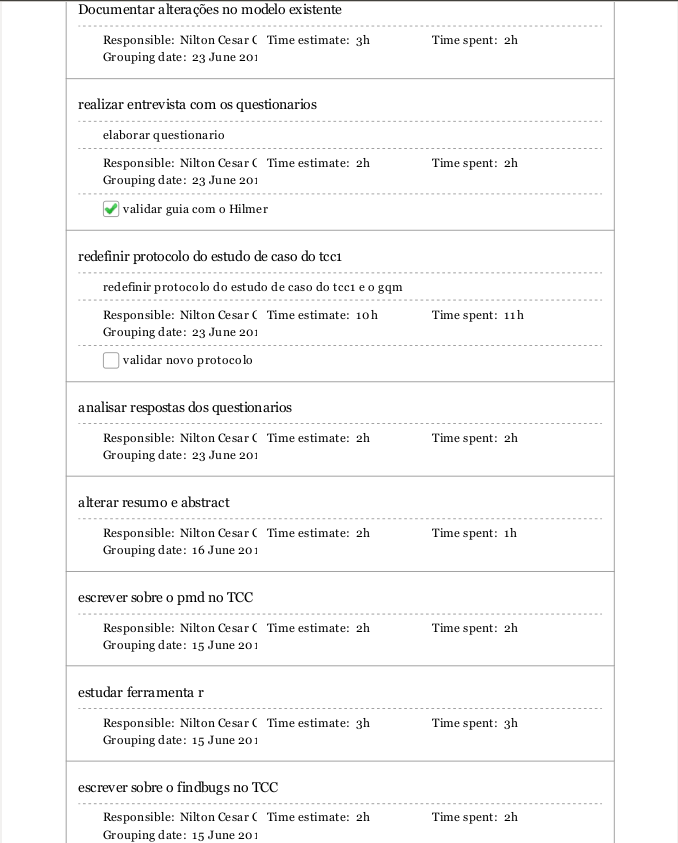
\includegraphics[keepaspectratio=false,scale=0.70]{figuras/figuras_nilton/kanban2.png}
\end{figure}

\begin{figure}[h!]
\centering
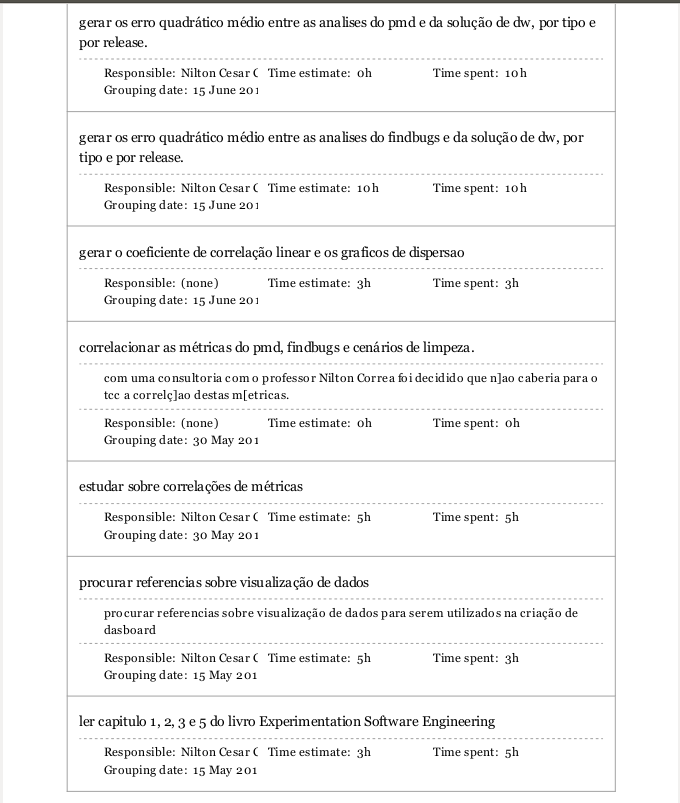
\includegraphics[keepaspectratio=false,scale=0.70]{figuras/figuras_nilton/kanban3.png}
\end{figure}

\begin{figure}[h!]
\centering
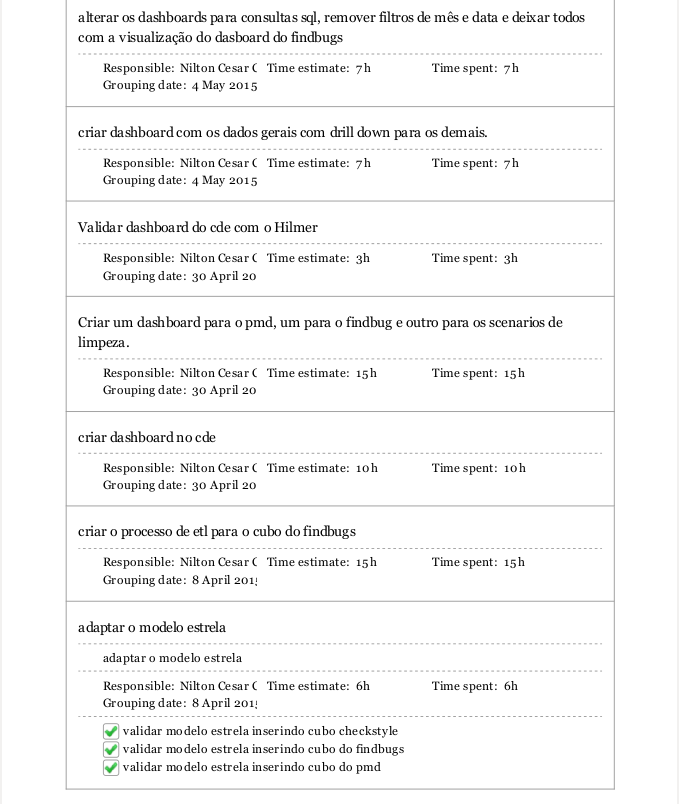
\includegraphics[keepaspectratio=false,scale=0.70]{figuras/figuras_nilton/kanban4.png}
\end{figure}

\begin{figure}[h!]
\centering
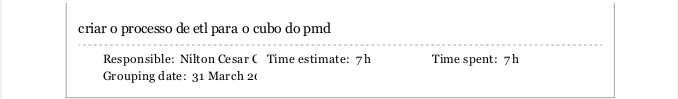
\includegraphics[keepaspectratio=false,scale=0.70]{figuras/figuras_nilton/kanban5.png}
\end{figure}




\chapter{Descrição do Processo de ETL no Kettle}
\label{sec:implementação-etl}

Neste apêndice, será apresentado a implementação do ETL no Kettle, onde se utilizou dos arquivos CSV resultantes da análise de métricas de código-fonte do Analizo, FindBugs e PMD.
No processo de ETL proposto por \citeonline{rego_monitoramento_2014TCC}, os arquivos do tipo CSV obtidos do Analizo foram convertidos para JSON, neste trabalho apenas os arquivos obtidos pelo Analizo e PMD foram convertidos para JSON, os arquivos obtidos do FindBugs foram mantidos no formado CSV. Visando realizar a conversão, foi escrito uma pequena aplicação \textit{web} na linguagem \textit{Ruby}, disponível para download no repositório do \textit{github} \footnote{https://github.com/matheustristao/csvto\_json}. 


\section{Implementações das \textit{Transformations}}


Como explicado anteriormente, o Kettle utiliza o componente de \textit{Transformation} para realizar cálculos, consultas em tabelas, inserções em tabelas, leitura de dados e entre outros. Os componentes que foram utilizados na solução de DW são mostrados na Figura \ref{fig:componentsetl}.


\begin{figure}[h!]
\centering
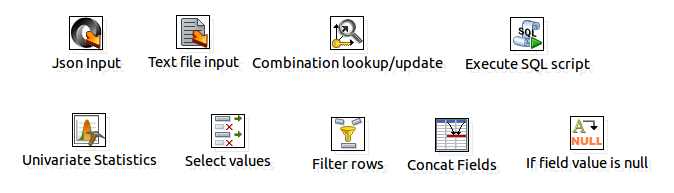
\includegraphics[keepaspectratio=false,scale=0.6]{figuras/figuras_nilton/componentsetl.png}
\caption{Componentes do Kettle que foram utilizadas nas Transformações}
\label{fig:componentsetl}
\end{figure}

O componente \textit{JSON Input} serve para ler os dados provenientes de um arquivo JSON, em que o conteúdo de cada variável pode ser lido como: \$..@nome\_da\_variavel. O componente \textit{Text file input} serve para o mesmo, porém para arquivos de outros tipos como o CSV.
O componente \textit{Univariate Statistics} é utilizado para se calcular estatísticas como média, mediana, número de amostras e percentis, que foram utilizados no cálculo dos intervalos percentis das métricas de código-fonte; O componente \textit{Execute SQL Script} foi utilizado para recuperação de dados no Metadados e Dimensões e também para inserção de nas Tabelas Fatos; O componente \textit{Combination Lookup} foi utilizado para se verificar se um determinado campo já existia em uma Dimensão, caso existisse, apenas se retornava o id da túpula, se não o inseria na Dimensão; O componente \textit{Select Values} foi utilizado para filtrar os dados provienente de outros componentes em uma \textit{Transformation}; O componente \textit{Filter rows} foi utilizado para que as linhas vazias dos arquivos fossem omitidas; O componente \textit{Concat Fields} foi utilizado para juntar os campos \textit{start} e \textit{end} da análise do FindBugs para formar o campo line que é padrão das outras análises; Por fim o componente \textit{if field is null} para rejeitar os valores de \textit{line} em branco.

Na primeira transformação, como se mostra na Figura \ref{fig:firsttransformation}, obtém-se os dados provinientes do arquivo JSON com componente \textit{JSON Input}. Em uma primeira etapa, coletava-se sobre dados: nome do projeto, release do arquivo, data de lançamento da release. Após a coleta dos dados do arquivo JSON, se inseria, conforme as verificações do componente \textit{Combination Lookup}, nas dimensões correspondentes.

\begin{figure}[h!]
\centering
\includegraphics[keepaspectratio=false,scale=0.65]{figuras/figuras_nilton/firsttransformation.eps}
\caption{Primeira Transformação realizada no Kettle}
\label{fig:firsttransformation}
\end{figure}
\FloatBarrier

Na segunda transformação, como se mostra na Figura \ref{fig:secondtransformation}, cobre-se o processo de negócio de avaliação dos valores percentis das métricas de código-fonte do projeto em uma determinada \textit{release} do software. Para tal, foi coletado os valores das métricas de código-fonte de cada classe com o componente \textit{JSON Input}. Após a coleta dos valores das métricas, esses eram direcionados ao componente \textit{Univariate Statistics} que realiza cálculos estatísticos. Após a realização dos cálculos, foi realizado um filtro com \textit{Select Values} a fim de se obter apenas os percentis obtidos para cada umas das métricas. 

\begin{figure}[h!]
\centering
\includegraphics[keepaspectratio=false,scale=0.65]{figuras/figuras_nilton/secondtransformation.eps}
\caption{Segunda Transformação realizada no Kettle}
\label{fig:secondtransformation}
\end{figure}
\FloatBarrier

Por fim, foi realizado a avaliação dos valores percentis, em intervalos qualitativos nos metadados com o componente \textit{Execute SQL Script}. Neste componente, recebeu-se o código-fonte descrito no Código-Fonte \ref{sqletlproject}, onde cada ? foi substituído por uma variável dentro da \textit{Transformation}.

\lstinputlisting[caption=\textit{Script} SQL de Avaliação dos Valores Percentis das Métricas de Código-Fonte, language=SQL, label=sqletlproject]{codigos/project-fact.sql}


Na terceira transformação, como se mostra na Figura \ref{fig:thirdtransformation}, foram cobertos os processos de negócio de avaliar os cenários de limpeza de código-fonte em cada classe do Projeto em uma determinada \textit{release} e o cálculo da Taxa de Aproveitamento de Oportunidades de Melhoria de Código-Fonte. Para tal, foram obtidos os valores cada métrica para cada classe utilizando o componente \textit{JSON Input}. Após a coleta das métricas, foram inseridas, utilizando o componente \textit{Combination Lookup} a fim de evitar duplicações ao longo das \textit{releases}, as classes do projeto.

\begin{figure}[h!]
\centering
\includegraphics[keepaspectratio=false,scale=0.65]{figuras/figuras_nilton/thirdtransformation.eps}
\caption{Terceira Transformação realizada no Kettle}
\label{fig:thirdtransformation}
\end{figure}
\FloatBarrier

Por fim, foram identificados os Cenários de Limpeza de Código-Fonte com auxílio dos metadados utilizando o componente \textit{Execute SQL Script}. Ainda neste componente, foi calculada a Taxa de Aproveitamento de Oportunidades de Melhoria de Código-Fonte a partir a soma de todos cenários de limpeza identificados em uma determinada release e a soma de todas as classes. O código-fonte, que foi colocado no componente \textit{Execute SQL Script} é descrito no Código-Fonte \ref{sqletlclass}, onde cada ? foi substituído por uma variável dentro da \textit{Transformation}.

\lstinputlisting[caption=\textit{Script} SQL de Identificação de Cenários de limpeza de Código-Fonte e Cálculo da Taxa de Aproveitamento de Oportunidades de Melhoria de Código-Fonte, language=SQL, label=sqletlclass]{codigos/classfact.sql}

Na quarta transformação, como se mostra na Figura \ref{fig:quartatransformation}, foram cobertos os processos de negócio para avaliar as violações do código-fonte em cada classe do Projeto em uma determinada \textit{release}. Para tal, foram obtidos os valores de cada violação para cada classe utilizando o componente \textit{JSON Input}. Após a coleta das violações, foram inseridas, utilizando o componente \textit{Combination Lookup} a fim de evitar duplicações ao longo das \textit{releases}, as classes do projeto.

\begin{figure}[h!]
\centering
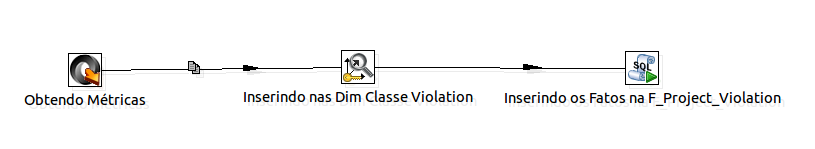
\includegraphics[keepaspectratio=false,scale=0.55]{figuras/figuras_nilton/quartatransformation.png}
\caption{Quarta Transformação realizada no Kettle}
\label{fig:quartatransformation}
\end{figure}
\FloatBarrier


Em seguida, foram identificados as violações do Código-Fonte e suas características utilizando o componente \textit{Execute SQL Script}.O código-fonte, que foi colocado no componente \textit{Execute SQL Script} é descrito no Código-Fonte \ref{sqletlviolacao}, onde cada ? foi substituído por uma variável dentro da \textit{Transformation}.


\lstinputlisting[caption=\textit{Script} SQL de Identificação das violações de Código-Fonte, language=SQL, label=sqletlviolacao]{codigos/sqletlviolacao.sql}

Na quinta transformação, como se mostra na Figura \ref{fig:quintatransformation}, foram cobertos os processos de negócio para avaliar \textit{bugs} do código-fonte em cada classe do Projeto em uma determinada \textit{release}. Para tal, foram obtidos os valores de cada \textit{bug} para cada classe utilizando o componente \textit{Text file Input}. Após a coleta dos \textit{bugs} foi utilizado o componente \textit{Filter rows} para desprezar as linhas em brancos do arquivo CSV, o componente \textit{If field value is null} para eliminar os os valores nulos dos campos \textit{start} e \textit{end} e o componete \textit{Concat Fields} para juntar os campos \textit{start} e \textit{end} em um único campo chamado \textit{line}. Em seguida, foram inseridas, utilizando o componente \textit{Combination Lookup} a fim de evitar duplicações ao longo das \textit{releases}, as classes do projeto.

\begin{figure}[h!]
\centering
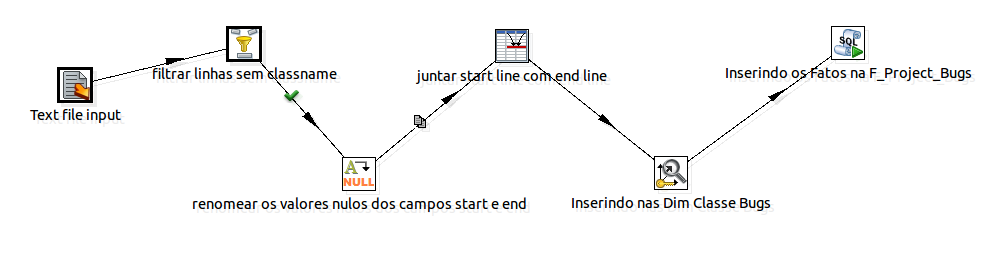
\includegraphics[keepaspectratio=true,scale=0.45]{figuras/figuras_nilton/quintatransformation.png}
\caption{Quinta Transformação realizada no Kettle}
\label{fig:quintatransformation}
\end{figure}
\FloatBarrier


Por fim, foram identificados \textit{bugs} do Código-Fonte e suas características utilizando o componente \textit{Execute SQL Script}.O código-fonte, que foi colocado no componente \textit{Execute SQL Script} é descrito no Código-Fonte \ref{sqletlbugs}, onde cada ? foi substituído por uma variável dentro da \textit{Transformation}.


\lstinputlisting[caption=\textit{Script} SQL de Identificação de \textit{bugs} no Código-Fonte, language=SQL, label=sqletlbugs]{codigos/sqletlbugs.sql}

\section{Implementação do \textit{Job}}

Como explicado anteriormente, o Kettle utiliza o  \textit{Job} para executar tarefas, em nível mais alto, de fluxo de controle, tais como, mandar um email em caso de falha, baixar um arquivo, executar transformações  e entre outras atividades. Dessa forma os principais componentes internos do \textit{Job}, que foram utilizados no trabalho, são mostrados na Figura \ref{fig:componentsjob}. 

\begin{figure}[h!]
\centering
\includegraphics[keepaspectratio=false,scale=0.60]{figuras/figuras_nilton/componentesjob.eps}
\caption{Componentes do Kettle que foram utilizadas nos \textit{Jobs}}
\label{fig:componentsjob}
\end{figure}
\FloatBarrier

O componente \textit{Start} é utilizado para marcar o início da execução de um determinado \textit{Job}. Nele, é possível programar a execução repetida de um determinado \textit{job}, como por exemplo, a cada hora, dia ou mês; O componente \textit{Transformation} serve para executar uma determinada Transformação, que fora especificada anteriormente. Já o componente \textit{set variables} serve para setar valores para variáveis que as transformações precisam para ser iniciada, neste trabalho foi criada uma variável que recebe o caminho dos arquivos das analises das ferramentas Analizo, FindBugs e PMD. 

Após se construir o arquivo \textit{Job} do presente trabalho, obteve-se a Figura \ref{fig:job}. 

\begin{figure}[h!]
\centering
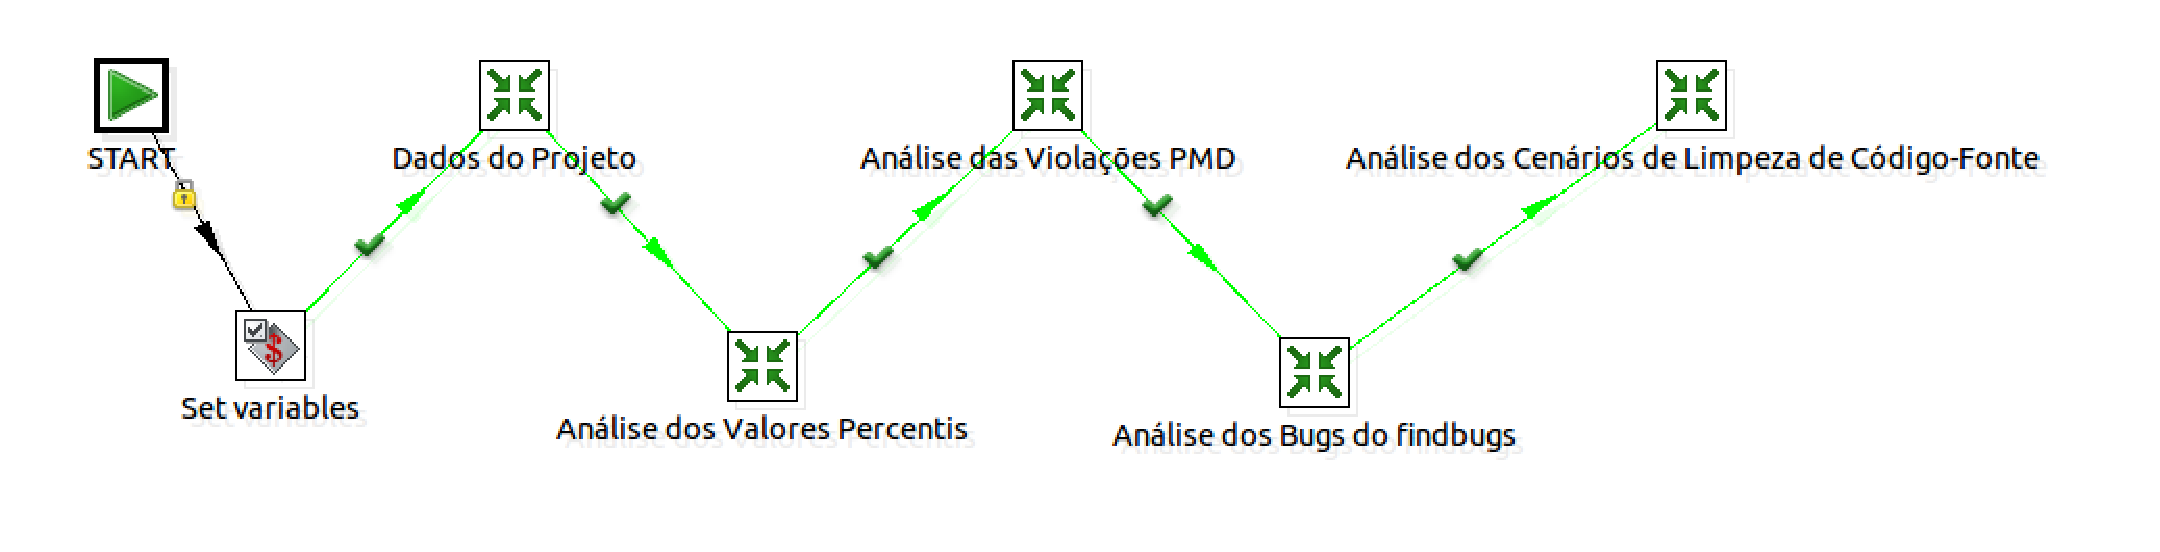
\includegraphics[keepaspectratio=false,scale=0.5]{figuras/figuras_nilton/job.eps}
\caption{\textit{Job} deste Trabalho}
\label{fig:job}
\end{figure}
\FloatBarrier

No \textit{Job}, a transformação~"Dados do Projeto"~corresponde a execução da Figura \ref{fig:firsttransformation}. Já a transoformação~"Análise dos Valores Percentis"~corresponde a Figura \ref{fig:secondtransformation}, a transformação~"Análise dos Cenários de Limpeza de Código-Fonte" corresponde a Figura \ref{fig:thirdtransformation}, a transoformação~"Análise das Violações PMD"~corresponde a Figura \ref{fig:quartatransformation} e por fim, a transoformação~"Análise dos Bugs do FindBugs"~corresponde a Figura \ref{fig:quintatransformation}.



\chapter{Implementação do \textit{Dashboard}}
\label{sec:implementação-dashboard}

\section{\textit{Dashboard} Geral}

Neste apêndice, será apresentado a implementação dos \textit{Dashboards} no CDE. O primeiro \textit{dashboard} a ser apresentado será o \textit{dashboard} Geral demonstrado na Figura \ref{fig:dashgeral}.

\begin{figure}[h!]
\centering
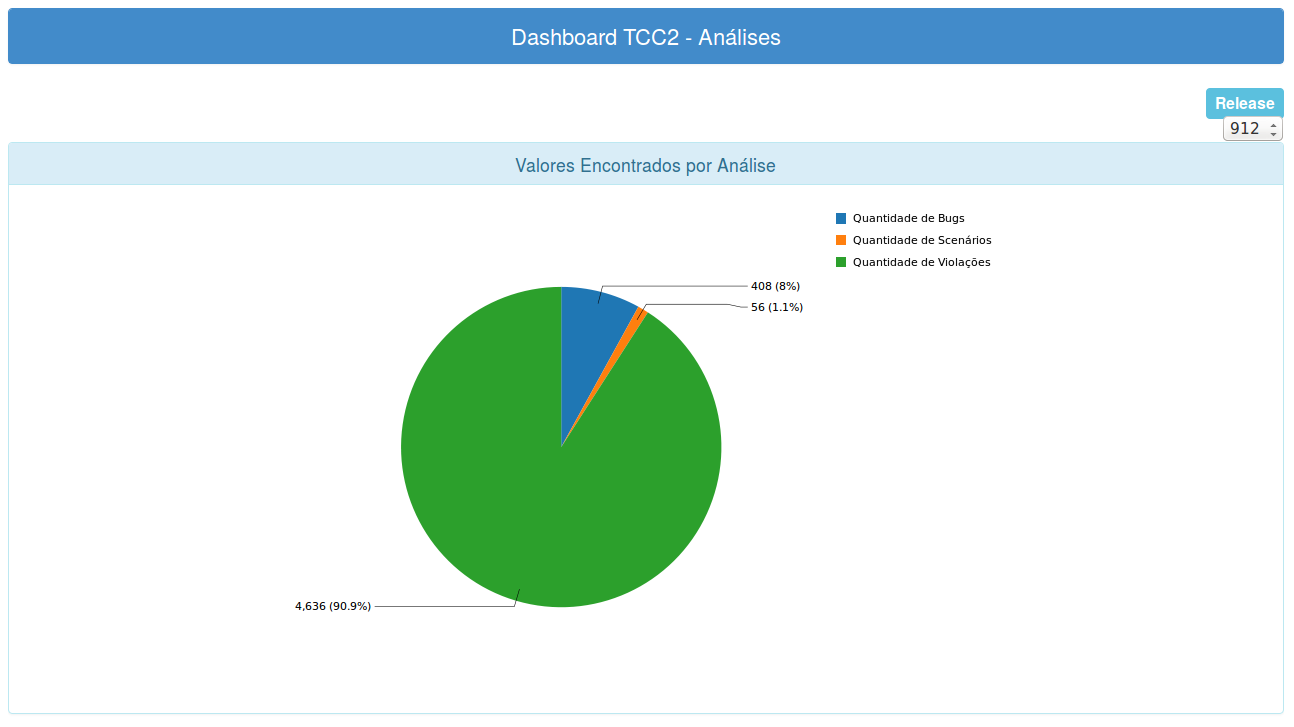
\includegraphics[keepaspectratio=false,scale=0.5]{figuras/figuras_nilton/dashgeral.png}
\caption{\textit{Dashboard} Geral}
\label{fig:dashgeral}
\end{figure}
\FloatBarrier

Como explicado anteriormente, o CDE oferece três perspectivas: \textit{Layout}, \textit{Components}, \textit{Datasources}. A estrutura  \textit{Layout} do {dashboard} Geral foi dividido em um \textit{Resource}, três \textit{Row} e quatro \textit{Column}. Dentro do \textit{Resource} foi escrito o código css abaixo:

{\color{blue}
\begin{verbatim}
body{
    margin-top: 0.5cm;
} 
paneltitle{
    vertical-align: top; 
}
.dashboardHeading{
     height:10px;
}

.releaseTextCss{
    /*top:-2px;*/  
    text-align:right;
} 
.releaseSelectorCss{
   /*top:-2px;*/  
    text-align:right;
}
.panel1Css{
    /*padding-right:30px;*/
    text-align: center;  
}
.panel2Css{
    padding-left:0px;
     text-align: center;  
}
.panel3Css{
     text-align: center;  
      overflow:auto; 
}

\end{verbatim}
}

A primeira \textit{Row} que define o nome do \textit{dashboard} na tela, possui um \textit{Column} com o código HTML abaixo:

{\color{blue}
\begin{verbatim}
<div class="panel panel-primary">
  <div class="panel-heading">Dashboard TCC2 - Análises</div>
</div> 
\end{verbatim}
}


A segunda \textit{Row}, possui duas \textit{Column} que definem o nome da \textit{release} com o código HTML abaixo e o \textit{selector} da \textit{release} que o utiliza a declaração \textit{releaseSelectorCss} do CSS.

{\color{blue}
\begin{verbatim}
<span class="label label-info" align="right">Release</span> 
\end{verbatim}
}

A última \textit{Row}, possui uma \textit{Column} que define o painel do gráfico \textit{pieChart} e possui o código HTML abaixo:

{\color{blue}
\begin{verbatim}
<div class="panel panel-info">
  <div class="panel-heading">
    <h3 class="panel-title">Valores Encontrados por Análise</h3>
  </div>
  <div class="panel-body" id="Panel3">
    Panel content
  </div>
</div> 
\end{verbatim}
}

A estrutura \textit{Components} foi dividido em três \textit{Groups}, \textit{Charts}, \textit{Generic} e \textit{Selects}. O \textit{Group} \textit{Charts} é responsavél pelo componente \textit{CCC pie Chart} que possui o código javascript abaixo e que possibilita o \textit{drill down} para os outros \textit{dashboards}.

{\color{blue}
\begin{verbatim}

function sendParameter(scene){
      var url = null;
       var urlPmd='http://localhost:8080/pentaho/api/repos/
       :public:dashboard:pmd:dashboard%20pmd%20v3.wcdf/generatedContent';
       var urlBug='http://localhost:8080/pentaho/api/repos/
       :public:dashboard:findbugs:dashboard%20fidbugs%20v3.wcdf
       /generatedContent';
       var urlScenarios='http://localhost:8080/pentaho/api/repos/
       :public:dashboard:scenarios:
       dashboard%20scenarios%20v3.wcdf/generatedContent';
       
       var vars = scene.vars;
       var c = vars.category.value;
       var v = vars.value.value;
       
       if (c == "Quantidade de Violações") {
         url = urlPmd;
         c = "PMD";
       }else if (c == "Quantidade de Bugs") {
         url = urlBug;
          c = "FindBugs";
       } else {
          url = urlScenarios;
           c = "Scenários de Limpeza";
       } 
       
       alert("análise:" + c + "\nquantidade: "+v);
      
       window.location=url;  
} 
\end{verbatim}
}

O \textit{Group} \textit{OLAP parameter} é responsável pela configuração do parâmetro utilizado para a construção do \textit{selector} da \textit{release} e possui o valor de propriedade abaixo:

{\color{blue}
\begin{verbatim}
[D Release.Release name].[All D Release.Release names]
\end{verbatim}
}

O \textit{Group} \textit{Select Component} é responsável pelas configurações do \textit{selector} da \textit{release}.

A perspectiva de \textit{Datasources} possui apenas o \textit{Group} \textit{MDX Queries} e possui duas consultas, a \textit{mdx over mondrianjndi} que é responsável pela consulta do gráfico \textit{CCC pie Chart} que é descrita abaixo:

{\color{blue}
\begin{verbatim}
with member [Measures].[Name] as '${release}.CurrentMember.UniqueName' 
select TopCount( filter({Descendants
([D Release.Release name].[All D Release.Release names] 
,[D Release.Release name]
.[Release name])}, not isempty(([D Release.Release name]
.CurrentMember)) ) , 50) on ROWS, 
 {[Measures].[Name]} on Columns 
 from [project violation]
\end{verbatim}
}

E a segunda consulta também é do tipo \textit{mdx over mondrianjn} e é responsável pela consulta do \textit{selector} da \textit{release} e está descrita abaixo:

{\color{blue}
\begin{verbatim}
WITH 
MEMBER [Measures].[Quantidade de Scenários] AS [Measures].[Quantiy Scenarios]
MEMBER [Measures].[Quantidade de Violações] AS [Measures].[Quantiy Violations]
MEMBER [Measures].[Quantidade de Bugs] AS [Measures].[Quantiy Bugs]
SELECT
NON EMPTY {Hierarchize({[D Project.Project abbreviation].
[Project abbreviation].Members})} ON COLUMNS,
NON EMPTY {Hierarchize({{[Measures].
[Quantidade de Scenários], [Measures].[Quantidade de Violações], 
[Measures].[Quantidade de Bugs]}})} ON ROWS
FROM [rate scenario]
WHERE {${release}}
\end{verbatim}
}


\section{\textit{Dashboards} Cenários, FindBugs e PMD}

Os \textit{Dashboards} Cenários, FindBugs e PMD que são apresentados nas Figuras \ref{dashcenario}, \ref{dashfindbugs} e \ref{dashpmd} possuem a perspectiva de \textit{layout} e \textit{Components} praticamente iguais mudando apenas as consultas na perspectiva de \textit{Datasources}.


A perspectiva de \textit{layout} dos três \textit{dashboards} foram divididos em um \textit{Resource}, quatro \textit{Row} e seis \textit{Column}. Dentro do \textit{Resource} foi escrito o código css abaixo:

{\color{blue}
\begin{verbatim}
body{
    margin-top: 0.5cm;
} 
paneltitle{
    vertical-align: top; 
}
.dashboardHeading{
     height:10px;
}

.releaseTextCss{
    /*top:-2px;*/  
    text-align:right;
} 
.releaseSelectorCss{
   /*top:-2px;*/  
    text-align:right;
}
.panel1Css{
    /*padding-right:30px;*/
    text-align: center;  
}
.panel2Css{
    padding-left:0px;
     text-align: center;  
}
.panel3Css{
     text-align: center;  
      overflow:auto; 
}

\end{verbatim}
}

\begin{figure}[H]
\centering
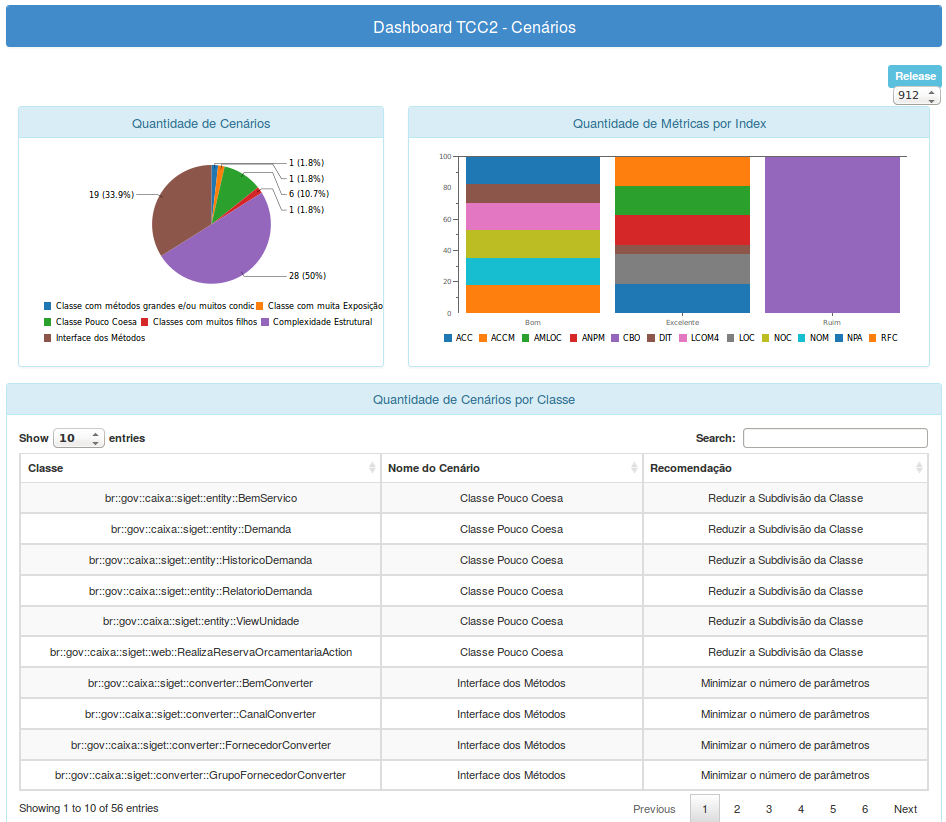
\includegraphics[keepaspectratio=false,scale=0.50]{figuras/figuras_nilton/dashcenario.png}
\caption{\textit{Dashboard} Cenários}
\label{dashcenario}
\end{figure}

\begin{figure}[H]
\centering
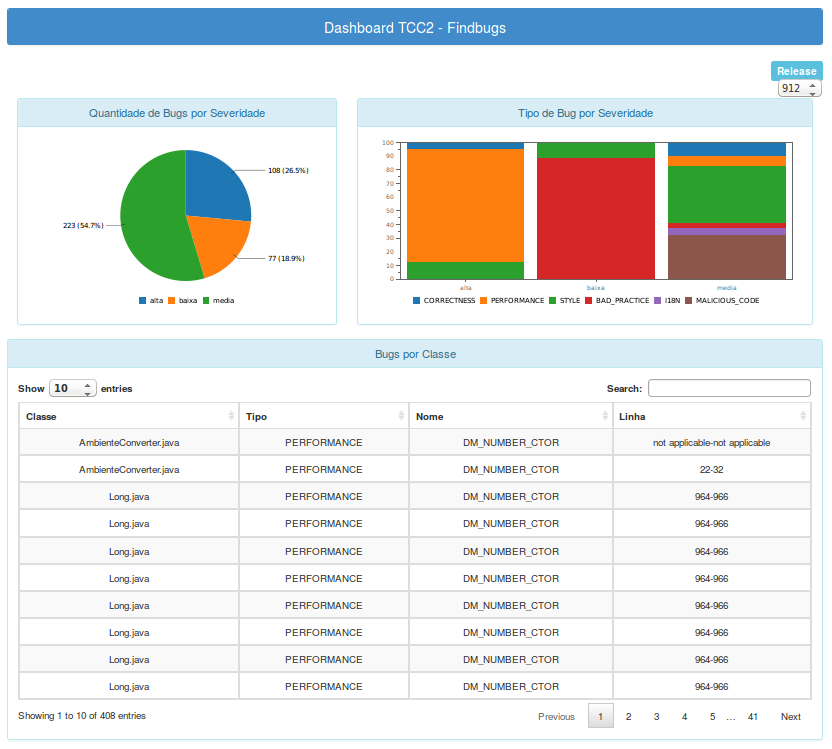
\includegraphics[keepaspectratio=false,scale=0.50]{figuras/figuras_nilton/DashboardFindbugs.png}
\caption{\textit{Dashboard FindBugs}}
\label{dashfindbugs}
\end{figure}

\begin{figure}[H]
\centering
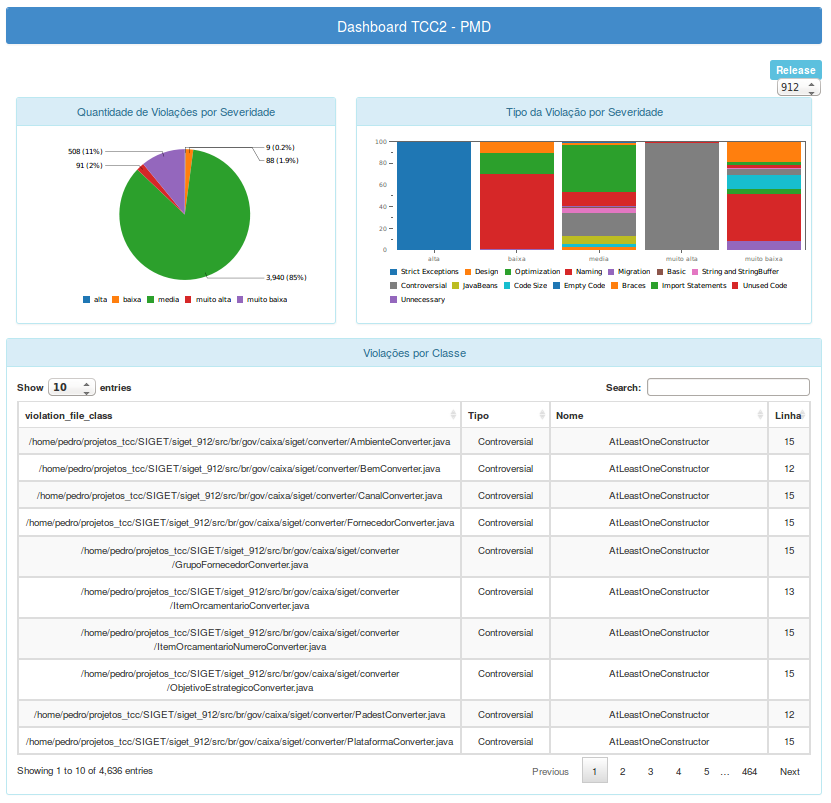
\includegraphics[keepaspectratio=false,scale=0.50]{figuras/figuras_nilton/DashboardPMD}
\caption{\textit{Dashboard} PMD}
\label{dashpmd}
\end{figure}


A primeira \textit{Row} que define o nome do \textit{dashboard} na tela, possui um \textit{Column} com um código HTML.

\textit{Dashboard Cenários}:
{\color{blue}
\begin{verbatim}
<div class="panel panel-primary">
  <div class="panel-heading">Dashboard TCC2 - Cenários</div>
</div> 
\end{verbatim} 
}

\textit{Dashboard Findbugs}:
{\color{blue}
\begin{verbatim}
<div class="panel panel-primary">
  <div class="panel-heading">Dashboard TCC2 - Findbugs</div>
</div> 
\end{verbatim} 
}

\textit{Dashboard PMD}:
{\color{blue}
\begin{verbatim}
<div class="panel panel-primary">
  <div class="panel-heading">Dashboard TCC2 - PMD</div>
</div> 
\end{verbatim} 
}

A segunda \textit{Row}, possui duas \textit{Column} que definem o nome da \textit{release} com o código HTML abaixo e o \textit{selector} da \textit{release} que o utiliza a declaração \textit{releaseSelectorCss} do CSS.

{\color{blue}
\begin{verbatim}
<span class="label label-info" align="right">Release</span> 
\end{verbatim}
}

A terceira \textit{Row}, possui duas \textit{Column}, a primeira define o painel do gráfico \textit{Pie Chart} e possui o código HTML abaixo:  

\textit{Dashboard Cenários}:
{\color{blue}
\begin{verbatim}
<div class="panel panel-info">
  <div class="panel-heading">
    <h3 class="panel-title">Quantidade de Cenários</h3>
  </div>
  <div class="panel-body" id="Panel1">
    Panel content
  </div>
</div> 
\end{verbatim}
}

\textit{Dashboard Findbugs}:
{\color{blue}
\begin{verbatim}
<div class="panel panel-info">
  <div class="panel-heading">
    <h3 class="panel-title">Quantidade de Bugs por Severidade</h3>
  </div>
  <div class="panel-body" id="Panel1">
    Panel content
  </div>
</div> 
\end{verbatim}
}

\textit{Dashboard PMD}:
{\color{blue}
\begin{verbatim}
<div class="panel panel-info">
  <div class="panel-heading">
    <h3 class="panel-title">Quantidade de Violaçôes por Severidade</h3>
  </div>
  <div class="panel-body" id="Panel1">
    Panel content
  </div>
</div> 
\end{verbatim}
}

e a segunda que define o painel do gráfico \textit{Stacked Bar Chart} e possui o código HTML abaixo: 


\textit{Dashboard Cenários}:
{\color{blue}
\begin{verbatim}
<div class="panel panel-info">
  <div class="panel-heading">
    <h3 class="panel-title">Quantidade de Métricas por Index</h3>
  </div>
  <div class="panel-body" id="Panel2">
    Panel content
  </div>
</div> 
\end{verbatim}
}

\textit{Dashboard Findbugs}:
{\color{blue}
\begin{verbatim}
<div class="panel panel-info">
  <div class="panel-heading">
    <h3 class="panel-title">Tipo de Bug por Severidade</h3>
  </div>
  <div class="panel-body" id="Panel2">
    Panel content
  </div>
</div> 
\end{verbatim}
}

\textit{Dashboard PMD}:
{\color{blue}
\begin{verbatim}
<div class="panel panel-info">
  <div class="panel-heading">
    <h3 class="panel-title">Tipo da Violação por Severidade</h3>
  </div>
  <div class="panel-body" id="Panel2">
    Panel content
  </div>
</div> 
\end{verbatim}
}

A última \textit{Row} define o painel do componente \textit{table Component} e possui o código HTML abaixo:

\textit{Dashboard Cenários}:
{\color{blue}
\begin{verbatim}
<div class="panel panel-info">
  <div class="panel-heading">
    <h3 class="panel-title">Quantidade de Cenários por Classe</h3>
  </div>
  <div class="panel-body" id="Panel3">
    Panel content
  </div>
</div> 

\end{verbatim}
}

\textit{Dashboard Findbugs}:
{\color{blue}
\begin{verbatim}
<div class="panel panel-info">
  <div class="panel-heading">
    <h3 class="panel-title">Bugs por Classe</h3>
  </div>
  <div class="panel-body" id="Panel3">
    Panel content
  </div>
</div> 
\end{verbatim}
}

\textit{Dashboard PMD}:
{\color{blue}
\begin{verbatim}
<div class="panel panel-info">
  <div class="panel-heading">
    <h3 class="panel-title">Violações por Classe</h3>
  </div>
  <div class="panel-body" id="Panel3">
    Panel content
  </div>
</div> 
\end{verbatim}
}

A estrutura \textit{Components} foi dividida em quatro \textit{Groups}, \textit{Charts}, \textit{Others}, \textit{Generic} e \textit{Selects}. O \textit{Group} \textit{Charts} é responsável pelos componentes \textit{CCC pie Chart} e \textit{CCC 100\% Stacked Bar Chart}; O \textit{Group} \textit{Others} é responsável pelo \textit{table Component}; \textit{Group} \textit{Generic} é responsável pela configuração do parâmetro utilizado para a construção do \textit{selector} da \textit{release}  e o \textit{Group} \textit{Selects} é responsável pelas configurações do \textit{selector} da \textit{release}.

A perspectiva de \textit{Datasources} possui apenas o \textit{Group} \textit{SQL Queries} e possui quatro consultas, todas do  tipo \textit{sql over sqljndi}. A primeira é responsável pela consulta do gráfico \textit{CCC pie Chart} e possuem consultas do tipo SQL que estão descritas abaixo:

\textit{Dashboard Cenários}:
{\color{blue}
\begin{verbatim}
select 
    dsc.scenario_name as "Nome do Cenário",
	sum(fsc.quantity_Scenario) as "Quantidade"
from
	F_Scenario_Class fsc,
	D_Release re,
	D_Scenario_Clean_Code dsc
where
	fsc.D_Scenario_Clean_Code_idScenario = dsc.idScenario
	and re.idRelease = fsc.D_Release_idRelease
	and re.release_name = ${release_param}
group by
	dsc.scenario_name
\end{verbatim}
}

\textit{Dashboard Findbugs}:
{\color{blue}
\begin{verbatim}
select 
    p.priority_name as "Prioridade", -- Para alterar o nome da 
    coluna basta alterar a string entre aspas
	sum(fpb.quantiy_Bug) as "Quantidade"
from 
	F_Project_Bug fpb,
	D_Priority p,
	D_Release re 
where	
	fpb.D_Class_Bug_idPriority = p.idPriority
	and re.idRelease = fpb.D_Release_idRelease
	and re.release_name = ${release_param} -- Colocar o parametro 
	com a release desejada aqui
group by 
	p.priority_name
\end{verbatim}
}

\textit{Dashboard PMD}:
{\color{blue}
\begin{verbatim}
select 
    s.severite_name as "Severidade",
	sum(fpv.quantiy_Violation) as "Quantidade"
from 
	F_Project_Violation fpv,
	D_Release re,
	D_Severite s
where
	fpv.D_Release_idRelease = re.idRelease
	and fpv.D_Class_Violation_idSeverite = s.idSeverite
	and re.release_name = ${release_param}
group by
	s.severite_name
\end{verbatim}
}

A segunda consulta é responsável pela consulta do componente \textit{CCC 100\% Stacked Bar Chart} e são descritas abaixo:

\textit{Dashboard Cenários}:
{\color{blue}
\begin{verbatim}
select 
    q.quality_index as "Index",
	m.metric_abbreviation as "Métrica"
	
from
	F_Project_Metric fpm,
	D_Release re,
	D_Metric m,
	D_Quality q
where
	fpm.D_Quality_idQuality = q.idQuality
	and fpm.D_Metric_idMetric = m.idMetric
	and re.idRelease = fpm.D_Release_idRelease
	and re.release_name = ${release_param} 
    group by
    q.quality_index,
    m.metric_abbreviation;
\end{verbatim}
}

\textit{Dashboard Findbugs}:
{\color{blue}
\begin{verbatim}
select
    p.priority_name as "Prioridade",
    t.type_category as "Tipo",
    sum(fpb.quantiy_Bug) as "Quantidade"
from 
	F_Project_Bug fpb,
	D_Priority p,
	D_Release re,
	D_Type t
where	
	fpb.D_Class_Bug_idPriority = p.idPriority
	and re.idRelease = fpb.D_Release_idRelease
	and fpb.D_Class_Bug_idType = t.idType
	and re.release_name = ${release_param} 
group by
    p.priority_name,
    t.type_category;
\end{verbatim}
}

\textit{Dashboard PMD}:
{\color{blue}
\begin{verbatim}
select 
    s.severite_name as "Severidade",
	r.rule_set as "Tipo",
	sum(fpv.quantiy_Violation) as "Quantidade"
from 
	F_Project_Violation fpv,
	D_Release re,
	D_Severite s,
	D_Rules r
where
    fpv.D_Class_Violation_idSeverite = s.idSeverite
	and re.idRelease = fpv.D_Release_idRelease
	and fpv.D_Class_Violation_idRules = r.idRules
	and re.release_name = ${release_param}
group by
	s.severite_name,
	r.rule_name;
\end{verbatim}
}

A terceira consulta é responsável pela consulta do \textit{table Component} e são descritas abaixo:

\textit{Dashboard Cenários}:
{\color{blue}
\begin{verbatim}
select  c.class_name as "Classe", dsc.scenario_name as "Nome do Cenário", 
dsc.recomendations as "Recomendação"

from D_Project pj, D_Release re, F_Scenario_Class fsc,
 D_Scenario_Clean_Code dsc, D_Class c

where

pj.idProject = fsc.D_Project_idProject 
and re.idRelease = fsc.D_Release_idRelease 
and fsc.D_Scenario_Clean_Code_idScenario = dsc.idScenario 
and c.idClass = fsc.D_Class_idClass
and re.release_name = ${release_param};
\end{verbatim}
}

\textit{Dashboard Findbugs}:
{\color{blue}
\begin{verbatim}
select  c.bug_file_class as "Classe", ty.type_category as "Tipo",
 ty.type_name as "Nome", c.bug_line_class as "Linha"

from  D_Class_Bug c, F_Project_Bug fpb, D_Type ty, 
D_Release re

where

c.idClass_bug = fpb.D_Class_Bug_idClass_Bug 
and ty.idType = fpb.D_Class_Bug_idType 
and re.idRelease = fpb.D_Release_idRelease
and re.release_name = ${release_param};
\end{verbatim}
}

\textit{Dashboard PMD}:
{\color{blue}
\begin{verbatim}
select
    dcv.violation_file_class,
	r.rule_set as "Tipo",
	r.rule_name as "Nome",
	dcv.violation_line_class as "Linha"
	
from 
	F_Project_Violation fpv,
	D_Release re,
	D_Severite s,
	D_Rules r,
	D_Class_Violation dcv
where
	fpv.D_Release_idRelease = re.idRelease
	and fpv.D_Class_Violation_idSeverite = s.idSeverite
	and fpv.D_Class_Violation_idRules = r.idRules
	and dcv.idClass_violation = fpv.D_Class_Violation_idClass_violation
	and re.release_name = ${release_param}
\end{verbatim}
}

A última consulta é responsável pela consulta do \textit{selector} da \textit{release} e são descritas abaixo:

\textit{Dashboard Cenários}:
{\color{blue}
\begin{verbatim}
select DISTINCT re.release_name

from D_Release re, F_Project_Metric fpm

where

re.idRelease = fpm.D_Release_idRelease;
\end{verbatim}
}

\textit{Dashboard Findbugs}:
{\color{blue}
\begin{verbatim}
select DISTINCT re.release_name

from D_Release re, F_Project_Bug fpb

where

re.idRelease = fpb.D_Release_idRelease;
\end{verbatim}
}

\textit{Dashboard PMD}:
{\color{blue}
\begin{verbatim}
select DISTINCT re.release_name

from D_Release re, F_Project_Violation fpv

where

re.idRelease = fpv.D_Release_idRelease;
\end{verbatim}
}

\chapter{Questionário}
\label{sec:questionário}

\begin{figure}[h!]
\centering

\includegraphics[keepaspectratio=false,scale=0.60]{figuras/figuras_nilton/questionario1.eps}
\label{questionario1}
\end{figure}

\begin{figure}[h!]
\centering
\includegraphics[keepaspectratio=false,scale=0.60]{figuras/figuras_nilton/questionario2.eps}
\label{questionario2}
\end{figure}

\begin{figure}[h!]
\centering
\includegraphics[keepaspectratio=false,scale=0.60]{figuras/figuras_nilton/questionario3.eps}
\label{questionario3}
\end{figure}


\begin{figure}[h!]
\centering
\includegraphics[keepaspectratio=false,scale=0.60]{figuras/figuras_nilton/questionario4.eps}
\label{questionario4}
\end{figure}


\end{apendicesenv}